\chapter{Solution Details}

Depth information is collected using the ARCore Raw Depth API via depth images and confidence images.
Low confidence points under a certain threshold are filtered out.
Each pixel of the depth image is then projected into three-dimensional world-space, utilizing the camera's intrinsics.
An octree is then use to remove duplicate points as new data arrives, and to quantize the points cloud.
The RANSAC algorithm is then applied to the point cloud to detect geometric primitives.


\section{Capturing Depth Images}

\subsection{Depth from Motion}
Depth from motion is a technique that estimates depth information from a sequence of images~\parencite{valentin_depth_2018}.

"Depth data becomes available when the user moves their device. The algorithm can get robust, accurate depth estimates from 0 to 65 meters away. The most accurate results come when the device is half a meter to about five meters away from the real-world scene. Experiences that encourage the user to move their device more will get better and better results."
\parencite{google_llc_arcore_doc}

\subsection{ARCore Depth APIs}
Google ARCore provides two APIs to access depth information: the Depth API and the Raw Depth API\@.
Both APIs provide depth information for a given frame of a camera image using depth images, but they differ in the level of detail they provide~\parencite{google_llc_arcore_doc}:

The Raw Depth API provides depth images and confidence images, where some pixels may not have any depth information.
The depth image provides the distance from the camera of a given pixel in millimeters.
The confidence image indicates the reliability of the depth information for each pixel, ranging from 0 (no confidence) to 255 (high confidence).

In contrast, the Depth API provides a single depth image, where each pixel has a depth value.
To achieve this, values for pixels without depth information are interpolated.
No confidence image is provided.

\begin{figure}[ht!]
    \centering
    % First row
    \begin{subfigure}[b]{0.4\textwidth}
        \centering
        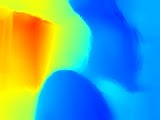
\includegraphics[width=0.8\linewidth]{images/depth_full-depth-image}
        \caption{Full Depth API depth image}
    \end{subfigure}%
    \begin{subfigure}[b]{0.4\textwidth}
        \centering
        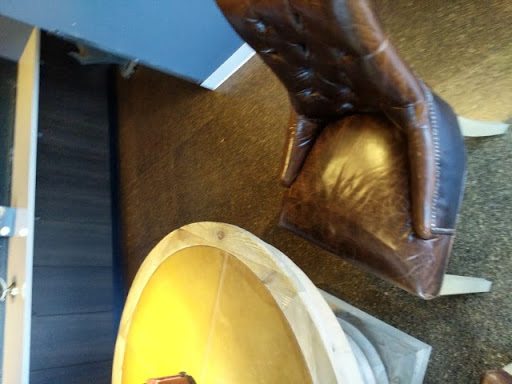
\includegraphics[width=0.8\linewidth]{images/depth_camera-image}
        \caption{Camera image}
    \end{subfigure}%

    % Optional: Adjust or remove vertical spacing between the rows
    \vspace{0.5em}

    % Second row
    \begin{subfigure}[b]{0.4\textwidth}
        \centering
        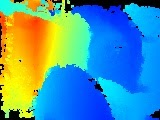
\includegraphics[width=0.8\linewidth]{images/depth_raw-depth-image}
        \caption{Raw Depth API depth image}
    \end{subfigure}%
    \begin{subfigure}[b]{0.4\textwidth}
        \centering
        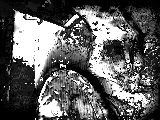
\includegraphics[width=0.8\linewidth]{images/depth_raw-depth-confidence-image}
        \caption{Raw Depth API confidence image}
    \end{subfigure}%

    \caption{Full Depth vs. Raw Depth}
    \label{fig:depth-api-images}
\end{figure}


The Depth API is preferred in cases where it is crucial to have a depth value for every pixel, such as calculating if an object should be occluded by the scene in an AR application,
while the Raw depth API is preferred if accuracy of the depth information is crucial. \parencite{google_llc_arcore_doc}
As accuracy is crucial for primitive detection and depth information for every pixel is not required, the Raw Depth API is used in this project.


\section{Building the point cloud (PC)}
As RANSAC is a point-based algorithm, we first need to convert the depth image to a point cloud.
The process consists of three steps.
\begin{enumerate}
    \item Filtering low confidence points
    \item Transforming depth image pixels to world coordinate points
    \item Inserting new points into the point cloud
\end{enumerate}

\subsection{Filtering low confidence points}
The confidence image provided by the Raw Depth API can be used to filter out points with low confidence.
A threshold value is set, below which points are discarded.

\subsection{Transforming depth image pixels to world coordinate points}
To convert the point into world coordinates, first the camera intrinsics are used to
project the point into camera space.
Then, the model matrix is used to transform the point into world space.
\parencite{google_llc_codelab_raw_depth,google_llc_arcore_doc}

These transformations can be seen as analog to the transformations needed to
render an object in world space onto the screen, as described in section~\ref{sec:rendering-the-primitives}.
In this case, the transformation is applied backwards, i.e.\ in the opposite direction of the arrows
in the figure~\ref{fig:coordinate-systems}, starting from screen space (5) to world space (2).
The parameters for the perspective projection matrix (section~\ref{sec:perspective-projection}) are derived from the camera intrinsics.


%"Given point $A$ on the observed real-world geometry and a 2D point a representing the same point in the depth image,
%the value given by the Depth API at a is equal to the length of $CA$ projected onto the principal axis.
%This can also be referred as the z-coordinate of $A$ relative to the camera origin $C$." \parencite{google_llc_arcore_doc}
%\begin{figure}[h]
%    \centering
%    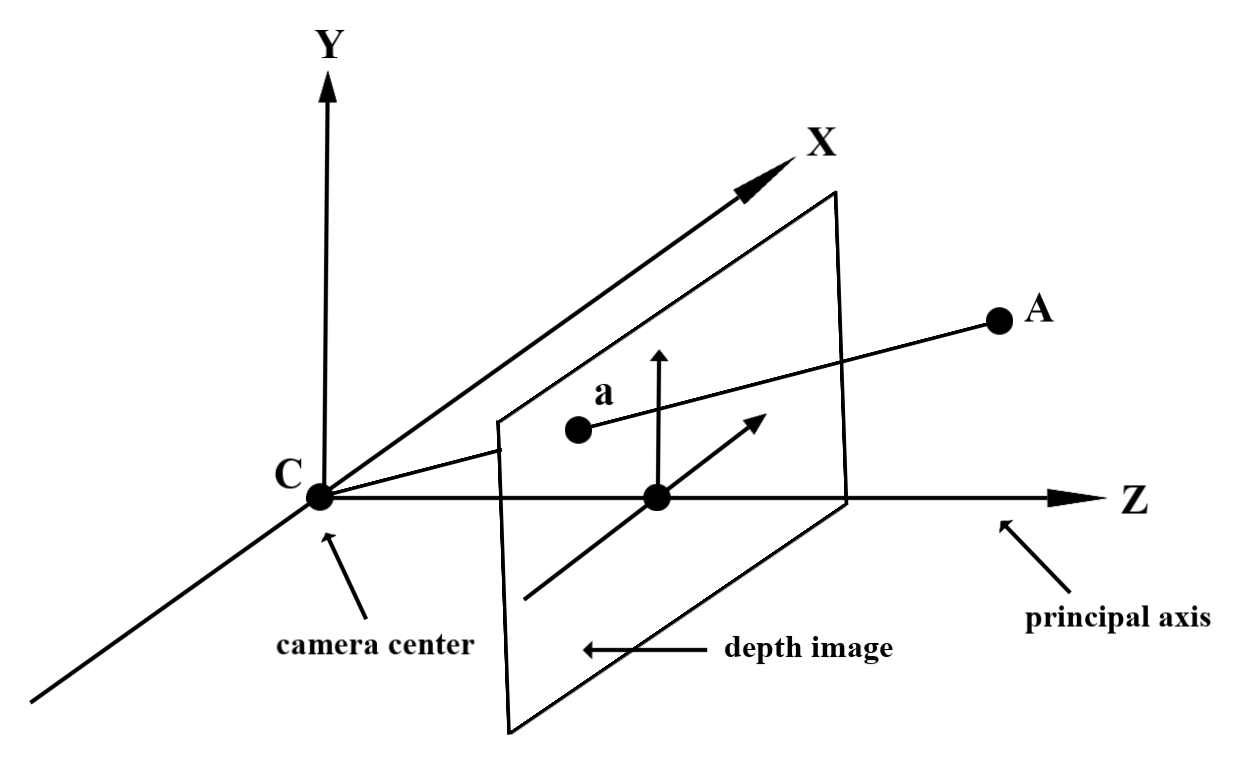
\includegraphics[width=0.75\textwidth]{images/depth-values-diagram}
%    \caption{}
%    \label{fig:}
%\end{figure}
%%codeblock with the formula
%\begin{lstlisting}[language=Java]
%float fx =
%  cameraTextureIntrinsics.getFocalLength()[0] * depthWidth / intrinsicsDimensions[0];
%float fy =
%  cameraTextureIntrinsics.getFocalLength()[1] * depthHeight / intrinsicsDimensions[1];
%float cx =
%  cameraTextureIntrinsics.getPrincipalPoint()[0] * depthWidth / intrinsicsDimensions[0];
%float cy =
%  cameraTextureIntrinsics.getPrincipalPoint()[1] * depthHeight / intrinsicsDimensions[1];
%pointCamera[0] = depthMeters * (x - cx) / fx;
%pointCamera[1] = depthMeters * (cy - y) / fy;
%pointCamera[2] = -depthMeters;
%pointCamera[3] = 1;
%\end{lstlisting}

%This results in a point in camera space,
%which can then be transformed into world space by multiplying it with the model matrix.

\subsection{Inserting new points into the point cloud}

The last step is to add new points to the point cloud.
As new depth images are captured every frame, we can not simply store a list of all points to append the new data to.
This would lead to a massive amount of points that represent the same point in space, with slightly different depth values.
To circumvent this, we can use a data structure that allows us to partition the space into smaller regions, and only store one point per region.
A simple approach would utilize a grid, where each cell represents a region in space, while a more sophisticated approach
would use a spatial data structure like an octree to improve performance.

\subsubsection{Octree}
An octree is a tree data structure where each node has exactly eight children.
The tree can be used to sparsely partition three-dimensional space into smaller cubes and allows for efficient
insertion and traversal in logarithmic time.
"For the definition a simple recursive splitting of [cubes] is continued until there is only one point in a [cube]."
\parencite{gabriel_zachmann_geometric_2002}

\begin{figure}[h]
    \centering
    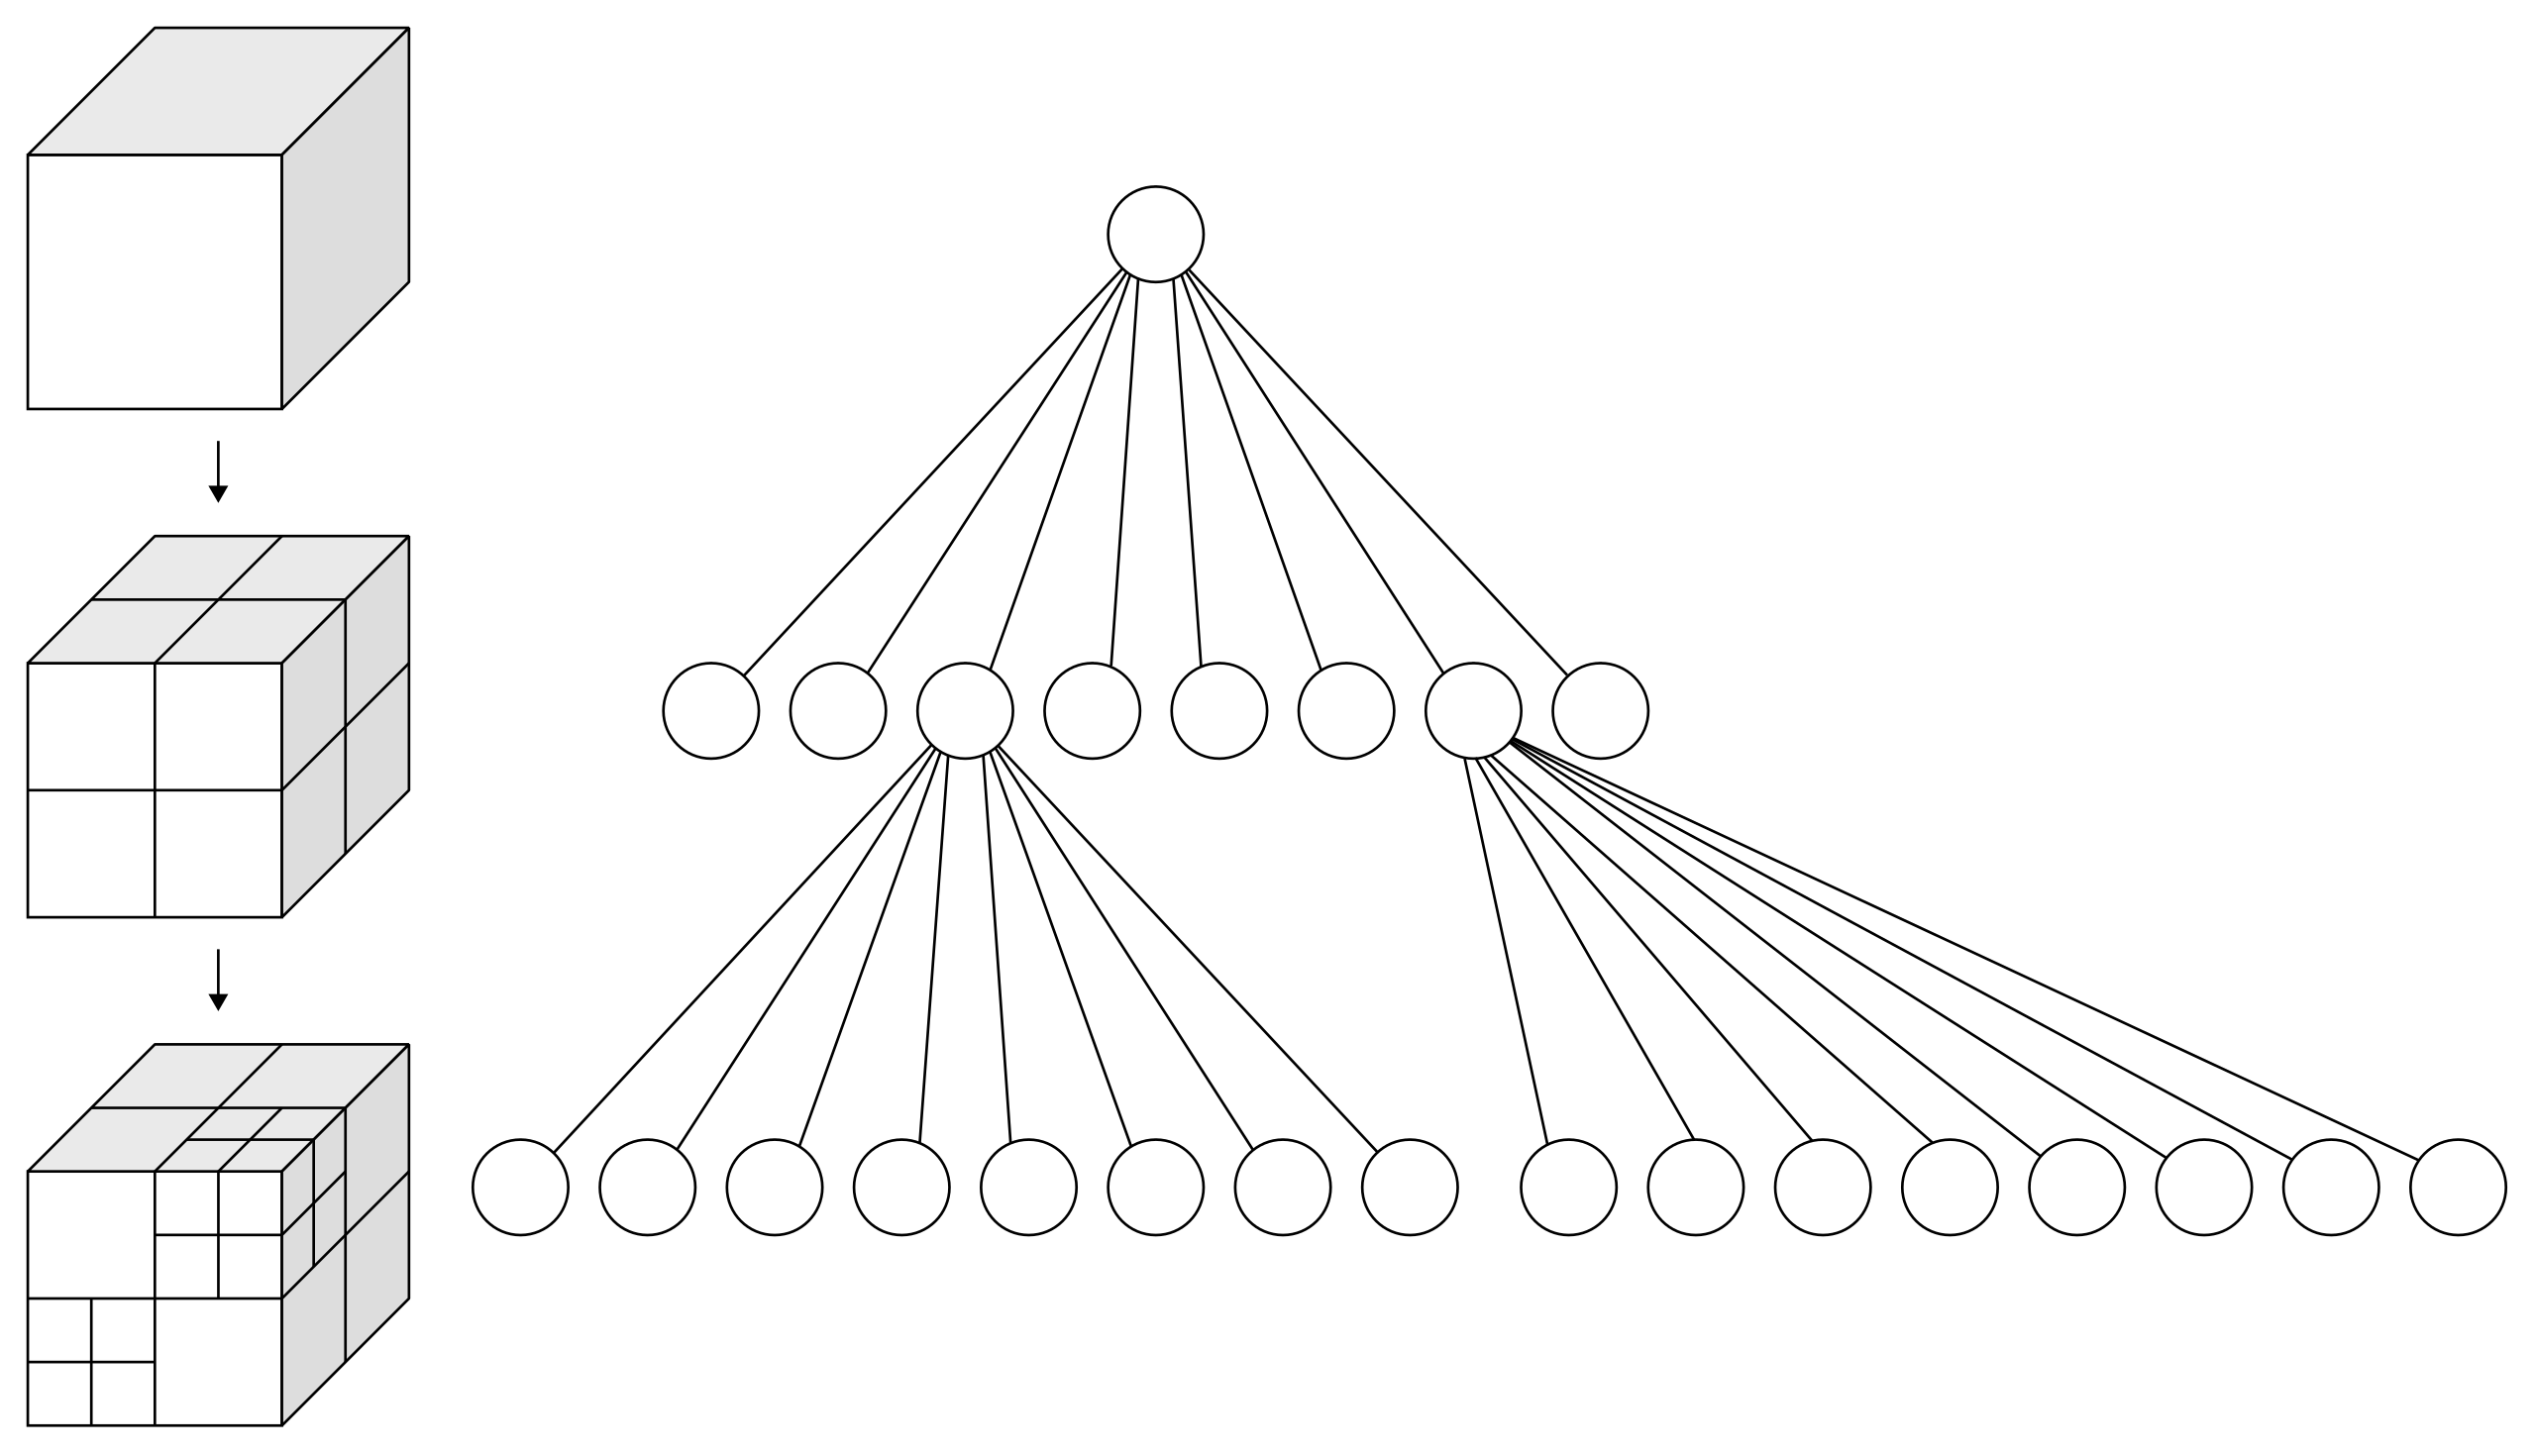
\includegraphics[width=0.75\textwidth]{images/octree}
    \caption{Octree}
    \label{fig:octrree}
\end{figure}

To utilize an octree for point cloud storage, the point coordinates and its data is saved in the leaf nodes of the octree.
In this case, each node of the octree saves the coordinate of the point and its confidence value.
When inserting a new point with a certain confidence value, a range query with a radius calculated from the confidence value
is performed to find all nodes within a certain distance of the point to be inserted.
If no node is found, a new leaf node is created and the point is inserted.
If a node is found with a lower confidence value, the new point is inserted and the old node is removed.
If a node is found with a higher confidence value, the new point is not inserted and discarded.
Using this approach, duplicate points are removed and adjusting the multiplier for the radius of the range query
allows for fine-tuning of the threshold under which points are considered duplicates.

A different approach is to use a variation of the octree with a fixed depth.
Points are always inserted at the defined depth of the tree, creating all nodes up to that depth if they do not yet exist.
The center coordinate of the leaf node can then be inferred as the point in space,
thus saving the coordinates of the point explicitly is not required.
Instead, to find the coordinates of a given node, the tree needs to be traversed while keeping track of
the extent and center coordinate of the current node.
This approach will naturally provide quantization of the point cloud, with the resolution of the point cloud
determined by the depth of the octree and extend of the root node.
Using this approach, duplicate points are removed and adjusting the resolution of the octree
allows for fine-tuning of the threshold distance between points under which points are considered duplicates.

One disadvantage of the latter approach is that the confidence value of the points are not considered,
thus a higher threshold for filtering out low confidence points is required.
This can be mitigated by extending the second approach by a technique similar to the first approach,
where the confidence value is stored with the point and a range query is performed to replace lower confidence values.

The performance of the RANSAC algorithm with both approaches will be evaluated in chapter~\ref{subsec:eval-point-clouds}.


\section{Detecting Primitives using RANSAC}

\parencite{schnabel_efficient_2007}


\section{Rendering the primitives}\label{sec:rendering-the-primitives}
The primitives are stored in world space, as in relative to the worlds' origin.
To render the primitives and overlay them onto the camera feed,
transforming the points from world space to screen space is required.

\subsection{OpenGL Rendering Pipeline}
This section provides an overview of the OpenGL rendering pipeline and the necessary steps to render the primitives.
All subsections are based on the book~\citetitle{de_vries_learn_2020} by \citeauthor{de_vries_learn_2020}~\parencite{de_vries_learn_2020}.

\subsubsection{Coordinate Systems}\label{subsec:coordinate-systems}
In OpenGL rendering, five coordinate systems are commonly used, as illustrated in figure~\ref{fig:coordinate-systems}.
In these coordinate systems, coordinates are relative to:
\begin{enumerate}
    \item the objects origin (\textit{Local Space})
    \item the worlds origin (\textit{World Space})
    \item the cameras origin (\textit{View Space})
    \item the cameras origin (\textit{Clip Space}) with visible coordinates between -1 and 1 in all dimensions (frustum).
    Coordinates outside the frustum are clipped.
    Perspective projection can be applied here, more details in the next subsection.
    \item the screen (\textit{Screen Space})  with the origin in the bottom left corner of the screen
\end{enumerate}
To transform vertices between these systems, their positions are multiplied with a corresponding transformation matrix.
One exception is the viewport transformation,
which is applied by OpenGL automatically based on the viewport settings provided via the \texttt{glViewport} function.

\begin{figure}[h!]
    \centering
    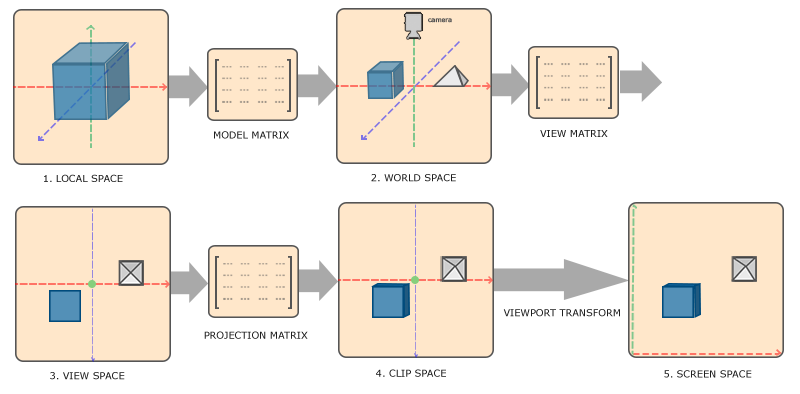
\includegraphics[width=\linewidth]{images/coordinate_systems}
    \caption{Coordinate systems}
    \label{fig:coordinate-systems}
\end{figure}

\subsubsection{Perspective Projection}\label{sec:perspective-projection}
In the real world, objects appear smaller the further away they are from the viewer.
To simulate this effect in 3D rendering, perspective projection is used.
Perspective projection is achieved through the use of homogeneous coordinates,
which are an extension of the Cartesian coordinate system.
In homogeneous coordinates, each point in 3D space is represented by four coordinates instead of three: $(x, y, z, w)$.

The transformation from 3D space to a 2D projection is handled by a projection matrix.
This matrix is designed to map the viewable scene, defined within a specified frustum, to a normalized cube known as clip space.
The frustum is a truncated pyramid shape that represents the volume of space visible through the camera lens.
The parameters of the frustum are defined by the field of view, aspect ratio, and near and far clipping planes,
as illustrated by figure~\ref{fig:perspective}
\begin{figure}[h]
    \centering
    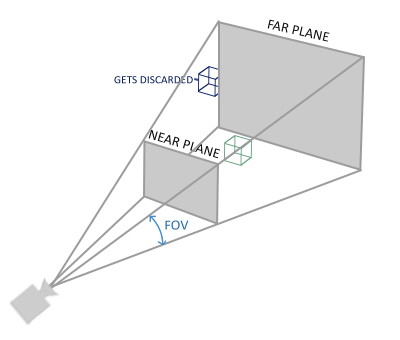
\includegraphics[width=0.50\textwidth]{images/perspective}
    \caption{Perspective Projection}
    \label{fig:perspective}
\end{figure}

"The projection matrix [\ldots] also manipulates the w value of each vertex coordinate in such a way
that the further away a vertex coordinate is from the viewer, the higher this w component becomes"~\parencite{de_vries_learn_2020}.
When the coordinates are later divided by $w$ (a process known as the perspective divide), %TODO QUOTAION NEEDED
it results in the desired perspective scaling effect.
Points closer to the viewer have a smaller $w$ and are less affected by the divide,
while points further away have a larger $w$ and are reduced in size more significantly

\subsubsection{Shaders}\label{subsec:shaders}
Shaders are isolated programs that run on the GPU and can be used to render objects.
In OpenGL, they are written in the OpenGL Shading Language (GLSL).

Two types of shaders are required to render an object: Vertex shaders and fragment shaders.

Vertex shaders are executed for each vertex defined in the vertex buffer, which is defined on the CPU and
passed to the GPU by copying the data to the GPU's memory, e.g.\ by using the \texttt{glBufferData} function.
A vertex shader can be used to transform the vertices from model space to screen space using the
model, view, and projection matrices.
To achieve this, the Model-View-Projection matrix (MVP) matrix can be passed as a \textit{uniform} to the vertex shader,
which means it is the same for all vertices.
The MVP matrix is the result of multiplying the model matrix, view matrix, and projection matrix.
As the MVP matrix is the same for all vertices of an object, it can be calculated on the CPU and passed to the GPU as a uniform.
The vertex position is then multiplied by the MVP matrix to transform it into clip space.
The resulting position is then passed to the fragment shader by assigning it to the \texttt{gl\_Position} variable.

\begin{figure}[h]
    \centering
    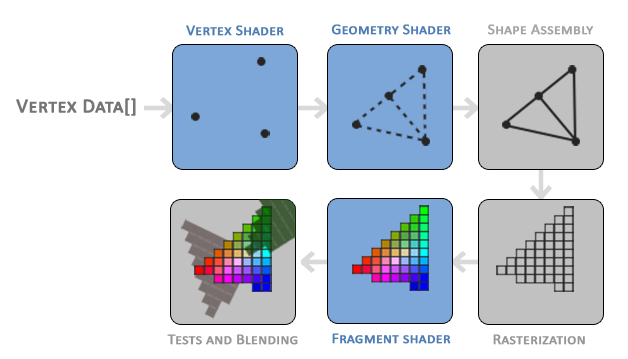
\includegraphics[width=0.70\textwidth]{images/graphics-pipeline}
    \caption{Graphics Pipeline. Blue boxes represent programmable stages. The Geometry Shader is optional and not covered in this thesis.}
    \label{fig:graphics-pipeline}
\end{figure}


The graphics pipeline then rasterizes and interpolates the vertex positions alongside all other vertex attributes
across the primitive, which are then passed to the fragment shader, which is executed for each pixel the primitive covers.
The fragment shader then outputs the color of the pixel by setting the \texttt{out vec4 FragColor} variable.
Before the final color is written to the framebuffer,
a depth test is performed to determine if the pixel is visible or covered by other pixels from other primitives.

\subsection{Rendering planes}
The RANSAC algorithm provides the parameterization of any detected plane using a normal vector $n$ and the point $p$ relative the worlds origin.
Using OpenGL, a plane can be rendered by creating two triangles composed of 3 vertices each, with two corner vertices shared between the triangles.
To render a plane from the parameterization, one can first find any two vectors $u$ and $v$
that are perpendicular to each-other and to the normal vector $n$.
Using $u$ and $v$, the four vertices of the plane can then be calculated by adding and subtracting $u * size / 2$ and $v * size / 2$ from the point $p$.

\paragraph{Calculating an arbitrary perpendicular vector}
The cross product of two vectors $a$ and $b$ is a vector that is perpendicular to both $a$ and $b$,
as long as $a$ and $b$ are not parallel.
To calculate an arbitrary perpendicular vector to a given vector $n$, one can use any of the 3 basis vectors ${b_1}$, ${b_2}$, and ${b_3}$.
Choosing any of the basis vectors that is not parallel to $n$ will result in a perpendicular vector.
To minimize floating point errors, which are largest for planes where $n$ almost aligns with the chosen basis vector,
the basis vector with the smallest dot product with $n$ can be chosen.
The normalized cross product of two vectors $n$ and $b_{smallest}$ then yields a perpendicular vector to $n$.

\begin{figure}[ht!]
    \centering
    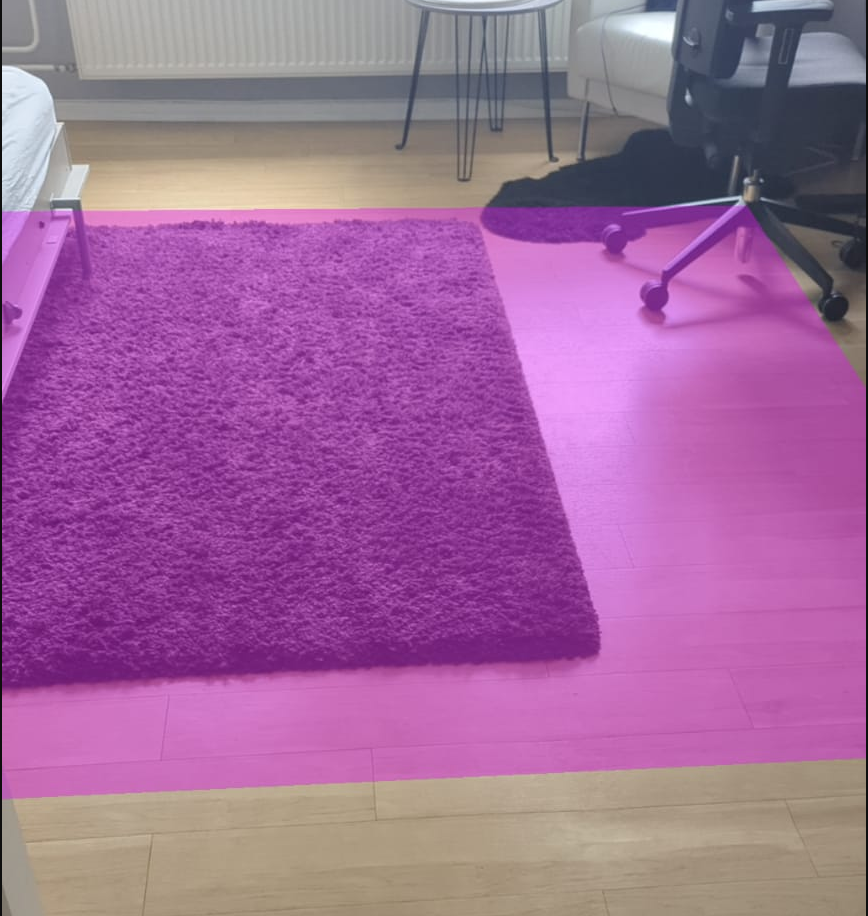
\includegraphics[width=0.6\linewidth]{images/renderedPlane}
    \caption{Rendered RANSAC plane with size of 2*2m}
\end{figure}

\subsection{Convex Hull}


\parencite{graham_efficient_1972}
\parencite{andrew_another_1979}

\subsection{Preparing the data on the CPU}

\subsubsection{Restraining the primitives}

\paragraph{Cross-section => Floor and Walls}

\paragraph{Using a bounding box / extend of points}

\subsubsection{Building a mesh}

\subsection{Rendering on the GPU (shaders)}
